\documentclass{report}

\usepackage[utf8]{inputenc} % For input encoding
\usepackage{amsmath}        % For mathematical formulas
\usepackage{graphicx}       % For including images
\usepackage{geometry}       % For page layout
\usepackage{float}
\usepackage{hyperref}      % For hyperlinks
\geometry{a4paper, margin=1in}

\title{A study place and a friendly penguin}
\author{\textbf{Owlgorithm} \\ Pinar Erbil, Angela Remolina, Duvan Diaz, and Camilo Sinning}
\date{\today}

\begin{document}

\maketitle

% \tableofcontents % Optional: adds a table of contents
\newpage

\begin{abstract}
In this report, we present our proposal developed for the Braynr track at the GDG hackathon. Our project, titled \textit{A Study Place and a Friendly Penguin}, envisions a comprehensive and interactive study environment powered by agentic AI. At the core of our concept is a virtual penguin assistant designed to guide and support students throughout their learning journey. This AI-driven agent interacts with users, provides personalized feedback, and adapts to individual study habits to maximize learning outcomes. By integrating features such as study planning, content organization, reminders, and gamified interactions within a single application, we aim to reinvent how students engage with their educational materials. Our approach emphasizes engagement, adaptability, and the use of intelligent agents to foster effective learning experiences.
\end{abstract}

\chapter{Introduction}

This is a report to describe our ideas about the Braynr track in the GDG hackaton.

\section{Current State}

The current state of the Braynr app is a desktop application that allows users to study and learn with the help of AI. The app is mainly focused on helping the students read and understand the content of their courses. 

\section{Proposed Challenge}
We needed to reimagine the app, trying to reinvent the way students learn and study. We wanted to create a more interactive and engaging experience for the users. The only thing we needed to take into account was the use of agentic AI, which is a type of AI that can act on its own and make decisions based on the data it receives.

\section{Proposed Solution}

Our proposal consists in creating an entire environment for study, we wanted the student to feel like when they are studying they only have to open an only app where they can do everything. We wanted to create a space where the student can study, play, and have fun. 

The central piece of our proposal is a friendly penguin that will be the guide of the student. The penguin will be the one who will help the student to study and learn. The penguin will be able to interact with the student and give them feedback on their progress. Also, the penguin will be aware of it's context and learn from the student. This penguin agent will have the only objective of getting the student to learn and study. So with the time it should learn the habits and methods that make you the most productive.

This penguin will have as it's content the whole app, and all it's integrated features, like the calendar, the notes, the reminders, and the study planner. The penguin will be able to interact with all these features and help the student to use them in a more efficient way.

We also will have some AI feature like the plan where the student will upload the content of it's course and through AI we will be able to generate a study plan for learning the content. This plan with contain questions and information making the student learn through and interactive process.

\footnotetext{Penguin animation credits: \url{https://giphy.com/pudgypenguins}}


\subsubsection{User Interface}

The figure~\ref{fig:ui} shows the landing page of the Braynr app.

\begin{figure}[H]
    \centering
    \begin{minipage}{0.48\textwidth}
        \centering
        
\includegraphics[width=\textwidth]{images/Home.png}
        \caption{Landing of the Braynr app}
        \label{fig:ui}
    \end{minipage}\hfill % \hfill fills the horizontal space
    \begin{minipage}{0.48\textwidth}
        \centering
        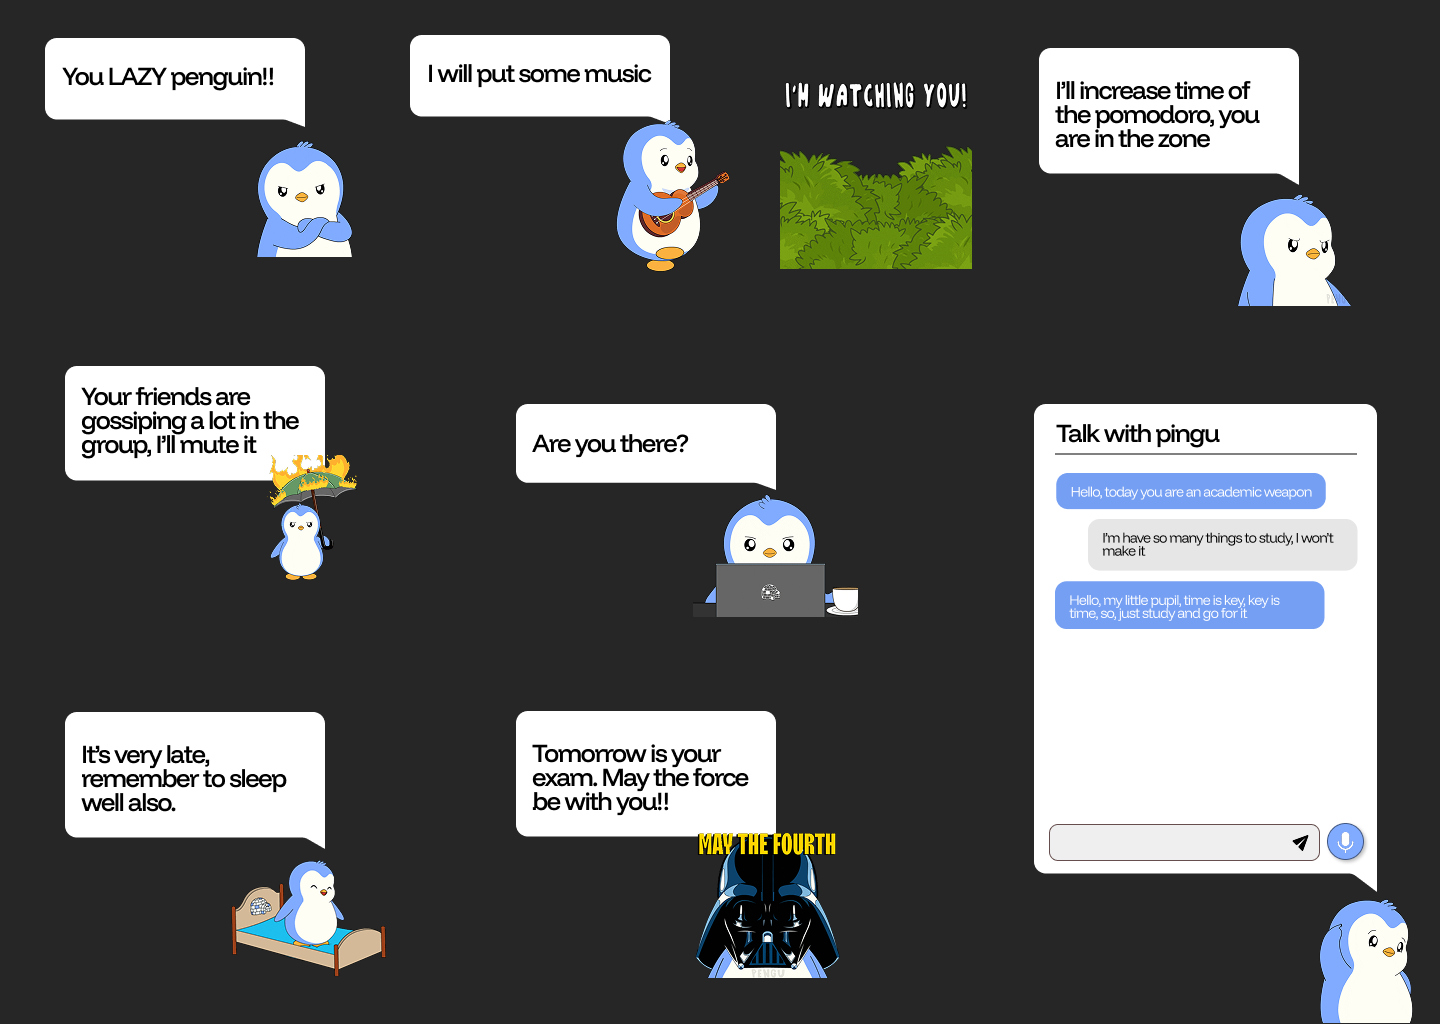
\includegraphics[width=\textwidth]{images/Pingu showcase.png}
        \caption{Penguin interacting with the user}
        \label{fig:chat}
    \end{minipage}
\end{figure}

Here are some examples of the penguin interacting with the user:

\section{Final thoughts and some technical details}
We think that this proposal is a good way to create a more interactive and engaging experience for the students. The penguin will be the perfect guide for the students, and it will help them to learn and study in a more efficient way. Our personalized penguin will work like a Reinforcement learner with a clear utility maximization (User learning).

How then do we define a utility function with something as abstract as learning? Our little penguin will sometimes ask the use questions about the content of the course, and based on the answers it will be able to have a rough idea of how much the user has learned. The penguin will also be able to ask the user about their preferences and habits, and based on that it will be able to create a personalized study plan for the user.

We are very excited about this proposal and we hope that you like it too.


\end{document}